\section{Supplemental Data}

\acused{CRT}
\begin{table}[htbp]
\centering
\begin{tabular}{l l m{2.2cm} m{3.0cm} m{3.0cm}}
\toprule
Session &
    Display &
        Video frame rate (\si{fps}) &
            Artefact Frequencies Removed (\si{Hz}) &
                Size of \SI{1}{\degree} square in visual field\\
\midrule
\sesname{H05391} &
    Projector &
        \raggedleft \num{30.015} &
            \num{30} &
                \SI{16.0 x 16.0}{px}\\
\sesname{H05nm7} &
    Projector &
        \raggedleft \num{30.015} &
            \num{30}, \num{60} &
                \SI{21.3 x 21.3}{px}\\
\sesname{H05nm9} &
    \ac{CRT} &
        \raggedleft \num{118.098} &
            ~ &
                \SI{17.8 x 17.9}{px}\\
\sesname{E07nm1} &
    \ac{CRT} &
        \raggedleft \num{118.098} &
            \num{50}, \num{150} &
                \SI{17.9 x 17.8}{px}\\
\sesname{F10nm1} &
    Projector &
        \raggedleft \num{30.015} &
            \num{30}, \num{60} &
                \SI{21.3 x 21.3}{px}\\
\sesname{J10nm1} &
    \ac{CRT} &
        \raggedleft \num{118.098} &
            ~ &
                \SI{17.8 x 17.9}{px}\\
\bottomrule
\end{tabular}
\caption{%
\textit{Metadata for recording sessions.}
Stimuli were presented using either an in-house custom-built projector (SVGA fibre-optic system with a resolution of \num{800x600} pixels; ``Projector''), or a cathode ray tube monitor (Iiyama MA203DT Vision Master Pro 513; ``\ac{CRT}'') placed at eye level, \SI{50}{\centi\metre} in front of the eye.
Videos presented at \SI{118}{Hz} were up-sampled versions of the original \SI{30}{Hz} video, which was achieved by repeating each frame four times.
For artefact removal methodology, see main text.
}
\label{tab:lam_md}
\end{table}


\begin{figure}
\centering 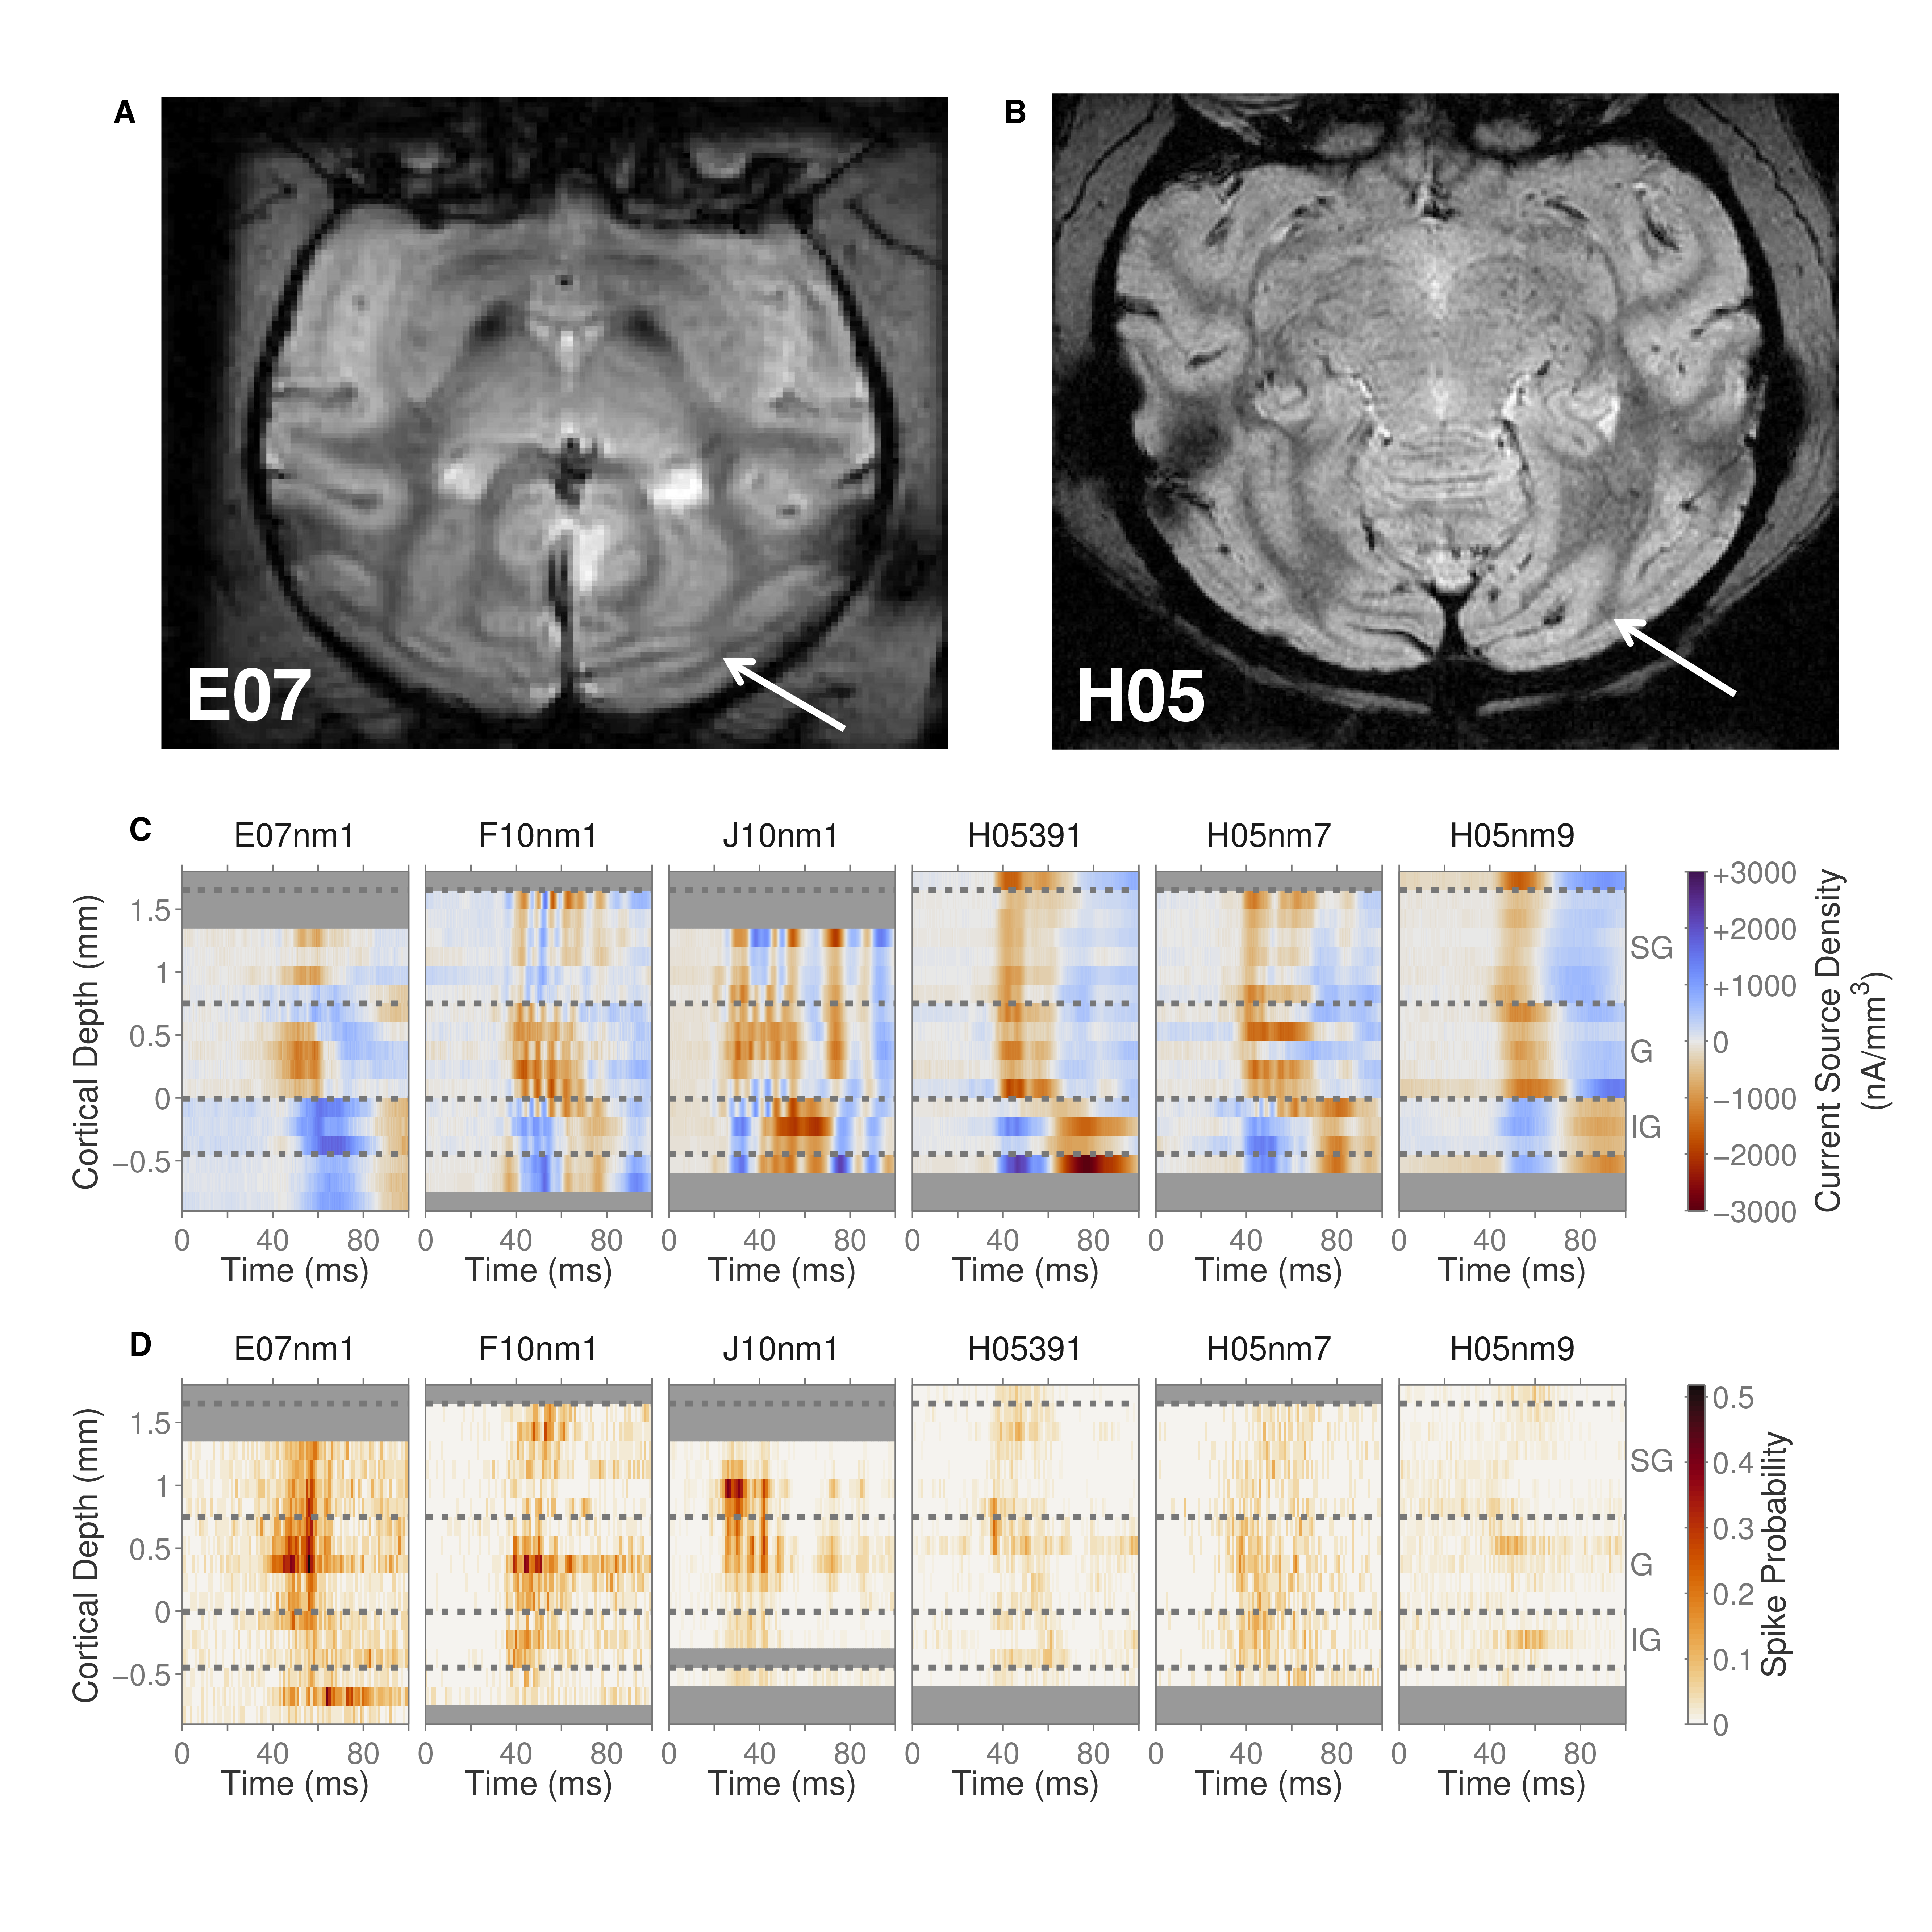
\includegraphics[width=\columnwidth]{paperfigs/figS1}
%
\caption{%
\textit{Electrode alignment.}
A--B: High resolution \ac{NMR} scans of two animals used to measure cortical thickness.
C: Stimulus triggered average \ac{CSD} responses, post-alignment.
For sessions \sesname{H05391}, \sesname{H05nm7}, \sesname{H05nm9} and \sesname{E07nm1}, the average response to onset of the movie stimulus is shown, whereas for sessions \sesname{F10nm1} and \sesname{J10nm1} the response to a full-field flash is shown.
D: Corresponding spike densities for the responses in panel C (\SI{1}{\milli\second} window duration).
}
\label{fig:lam_s1}
%
\end{figure}


\begin{figure}
\centering 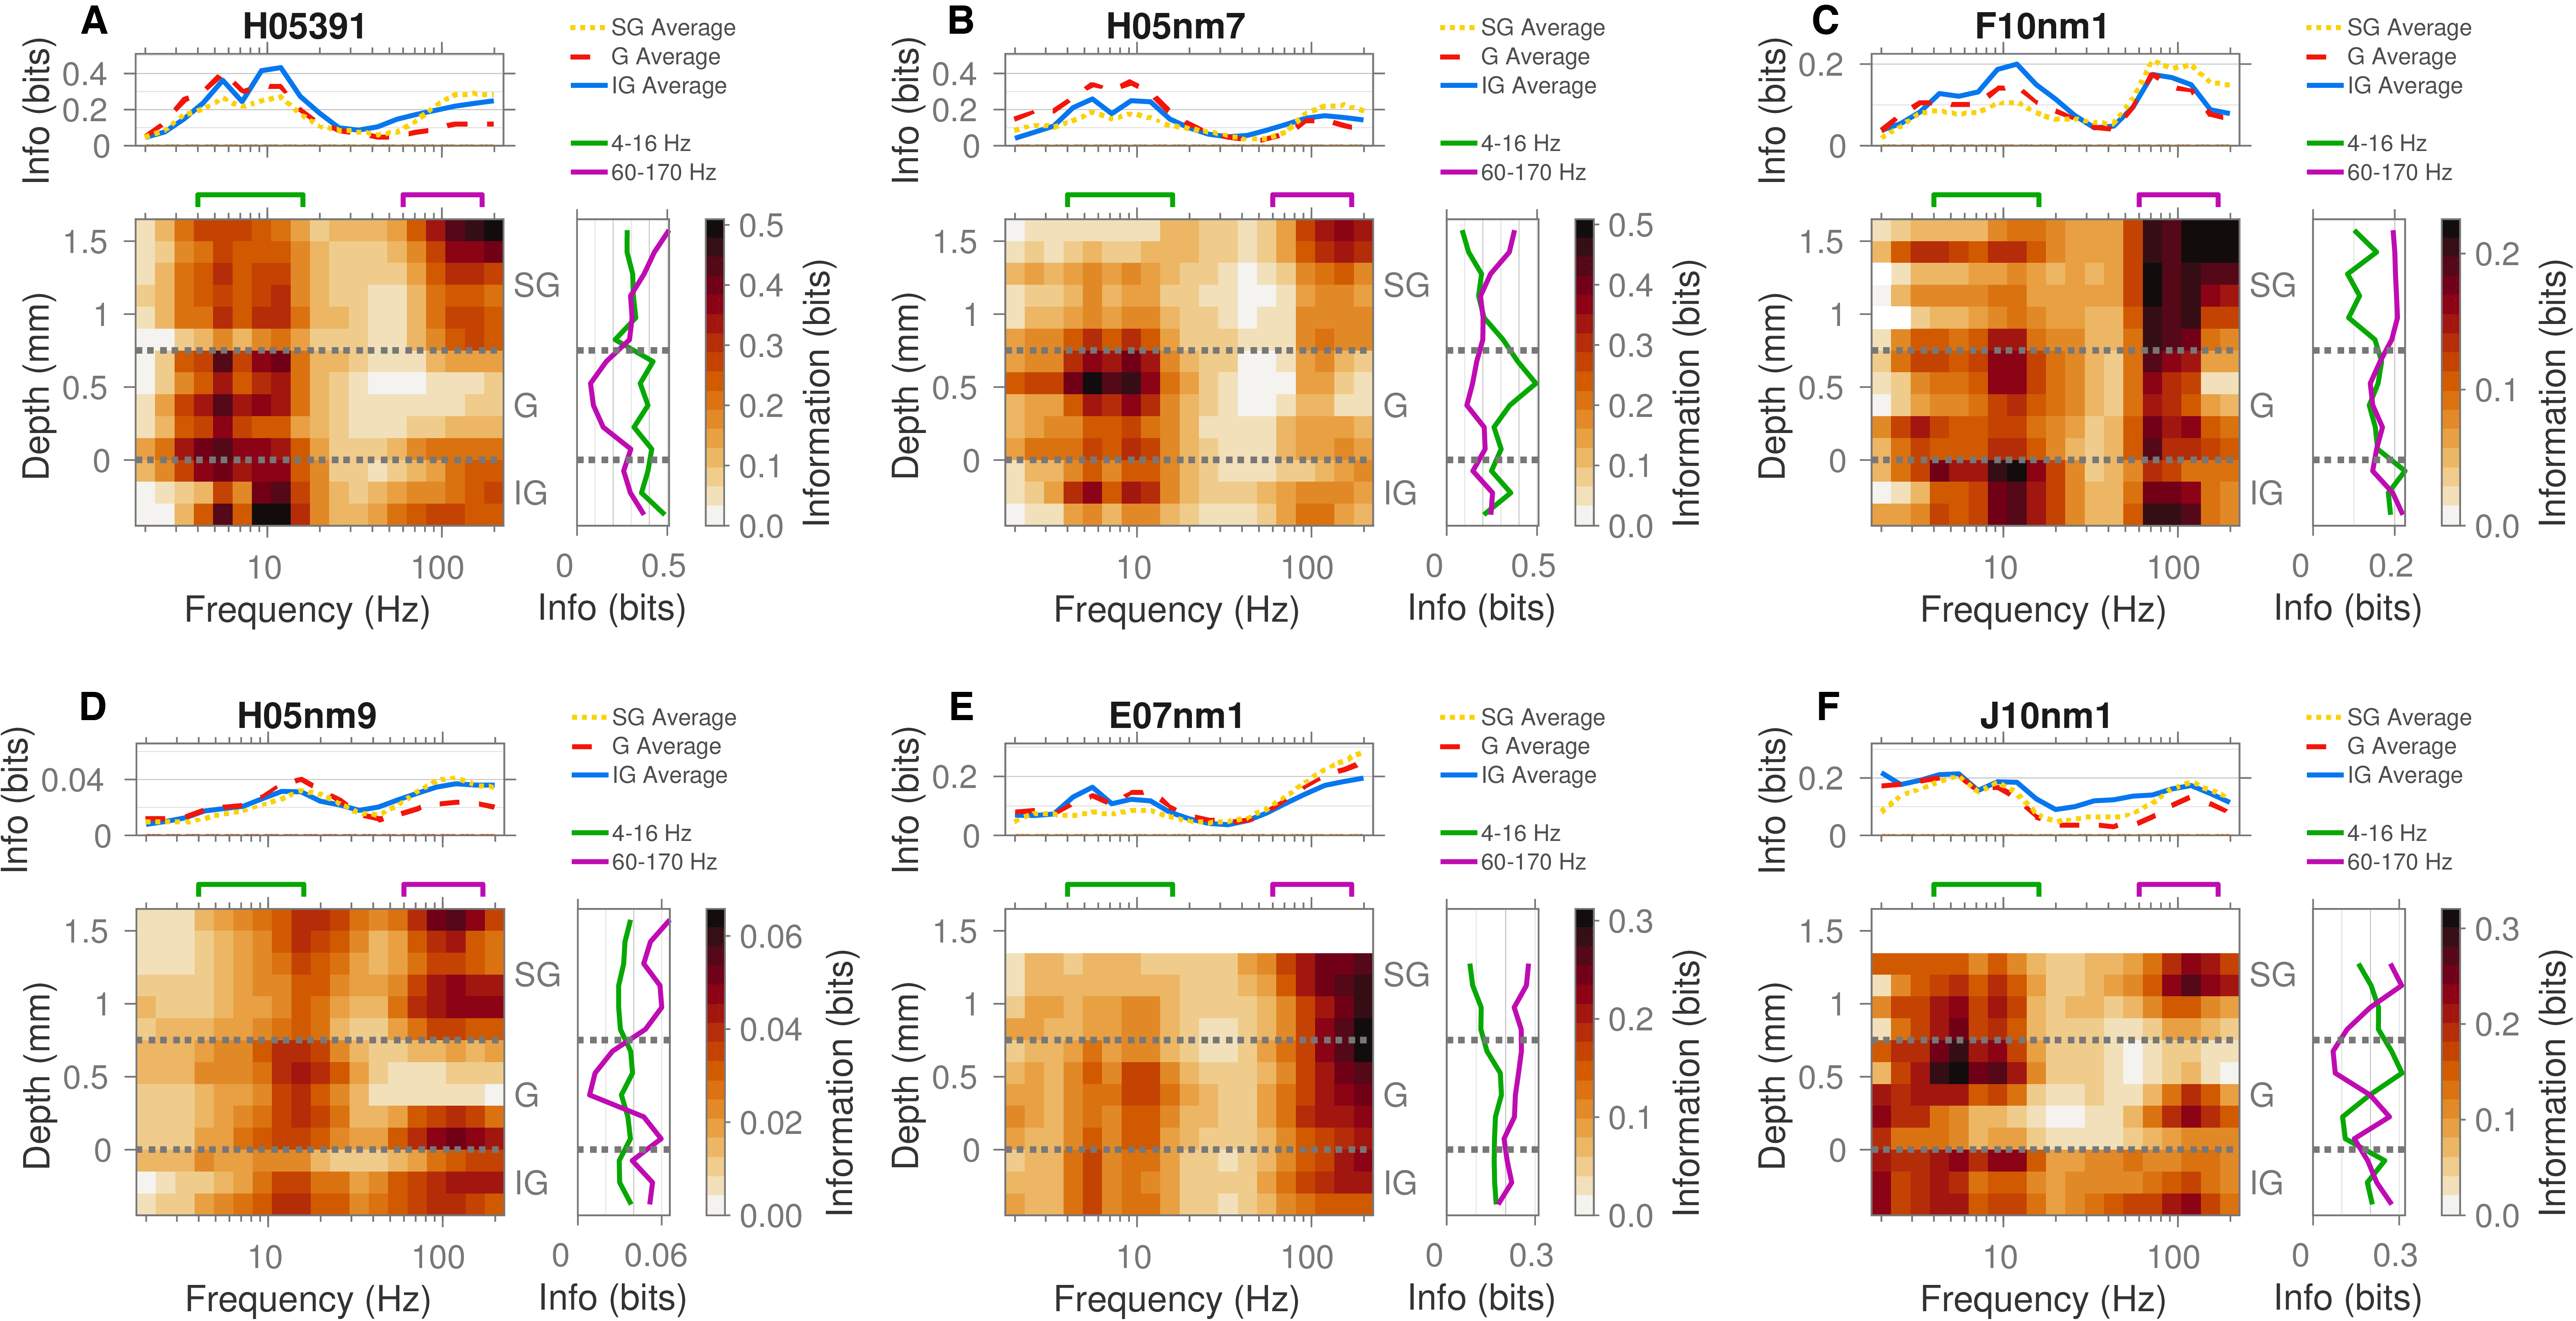
\includegraphics[width=\columnwidth]{paperfigs/figS2}
%
\caption{%
\textit{Distribution of information about the movie across both cortical depth and frequency for individual sessions}
A--F: Same as \autoref{fig:lam_2}D, but shown for each recording session individually.
Distribution of information about movie stimulus contained in power.
Each datapoint was tested for statistical significance using bootstrapping; for each depth and frequency band in each session a significance threshold was set at 3 standard deviations of the bootstrap distribution.
The median threshold for significance across all frequencies and depths is indicated by a line on each colour bar.
Non-significant values are shown in white.
Above each, mean information within \ac{SG}, \ac{G} and \ac{IG} compartments.
Right of each, cortical distribution of information in the power of two frequency bands; \SIrange{4}{16}{Hz} and \SIrange{60}{170}{Hz}.
}
\label{fig:lam_s2}
%
\end{figure}


\begin{figure}
\centering 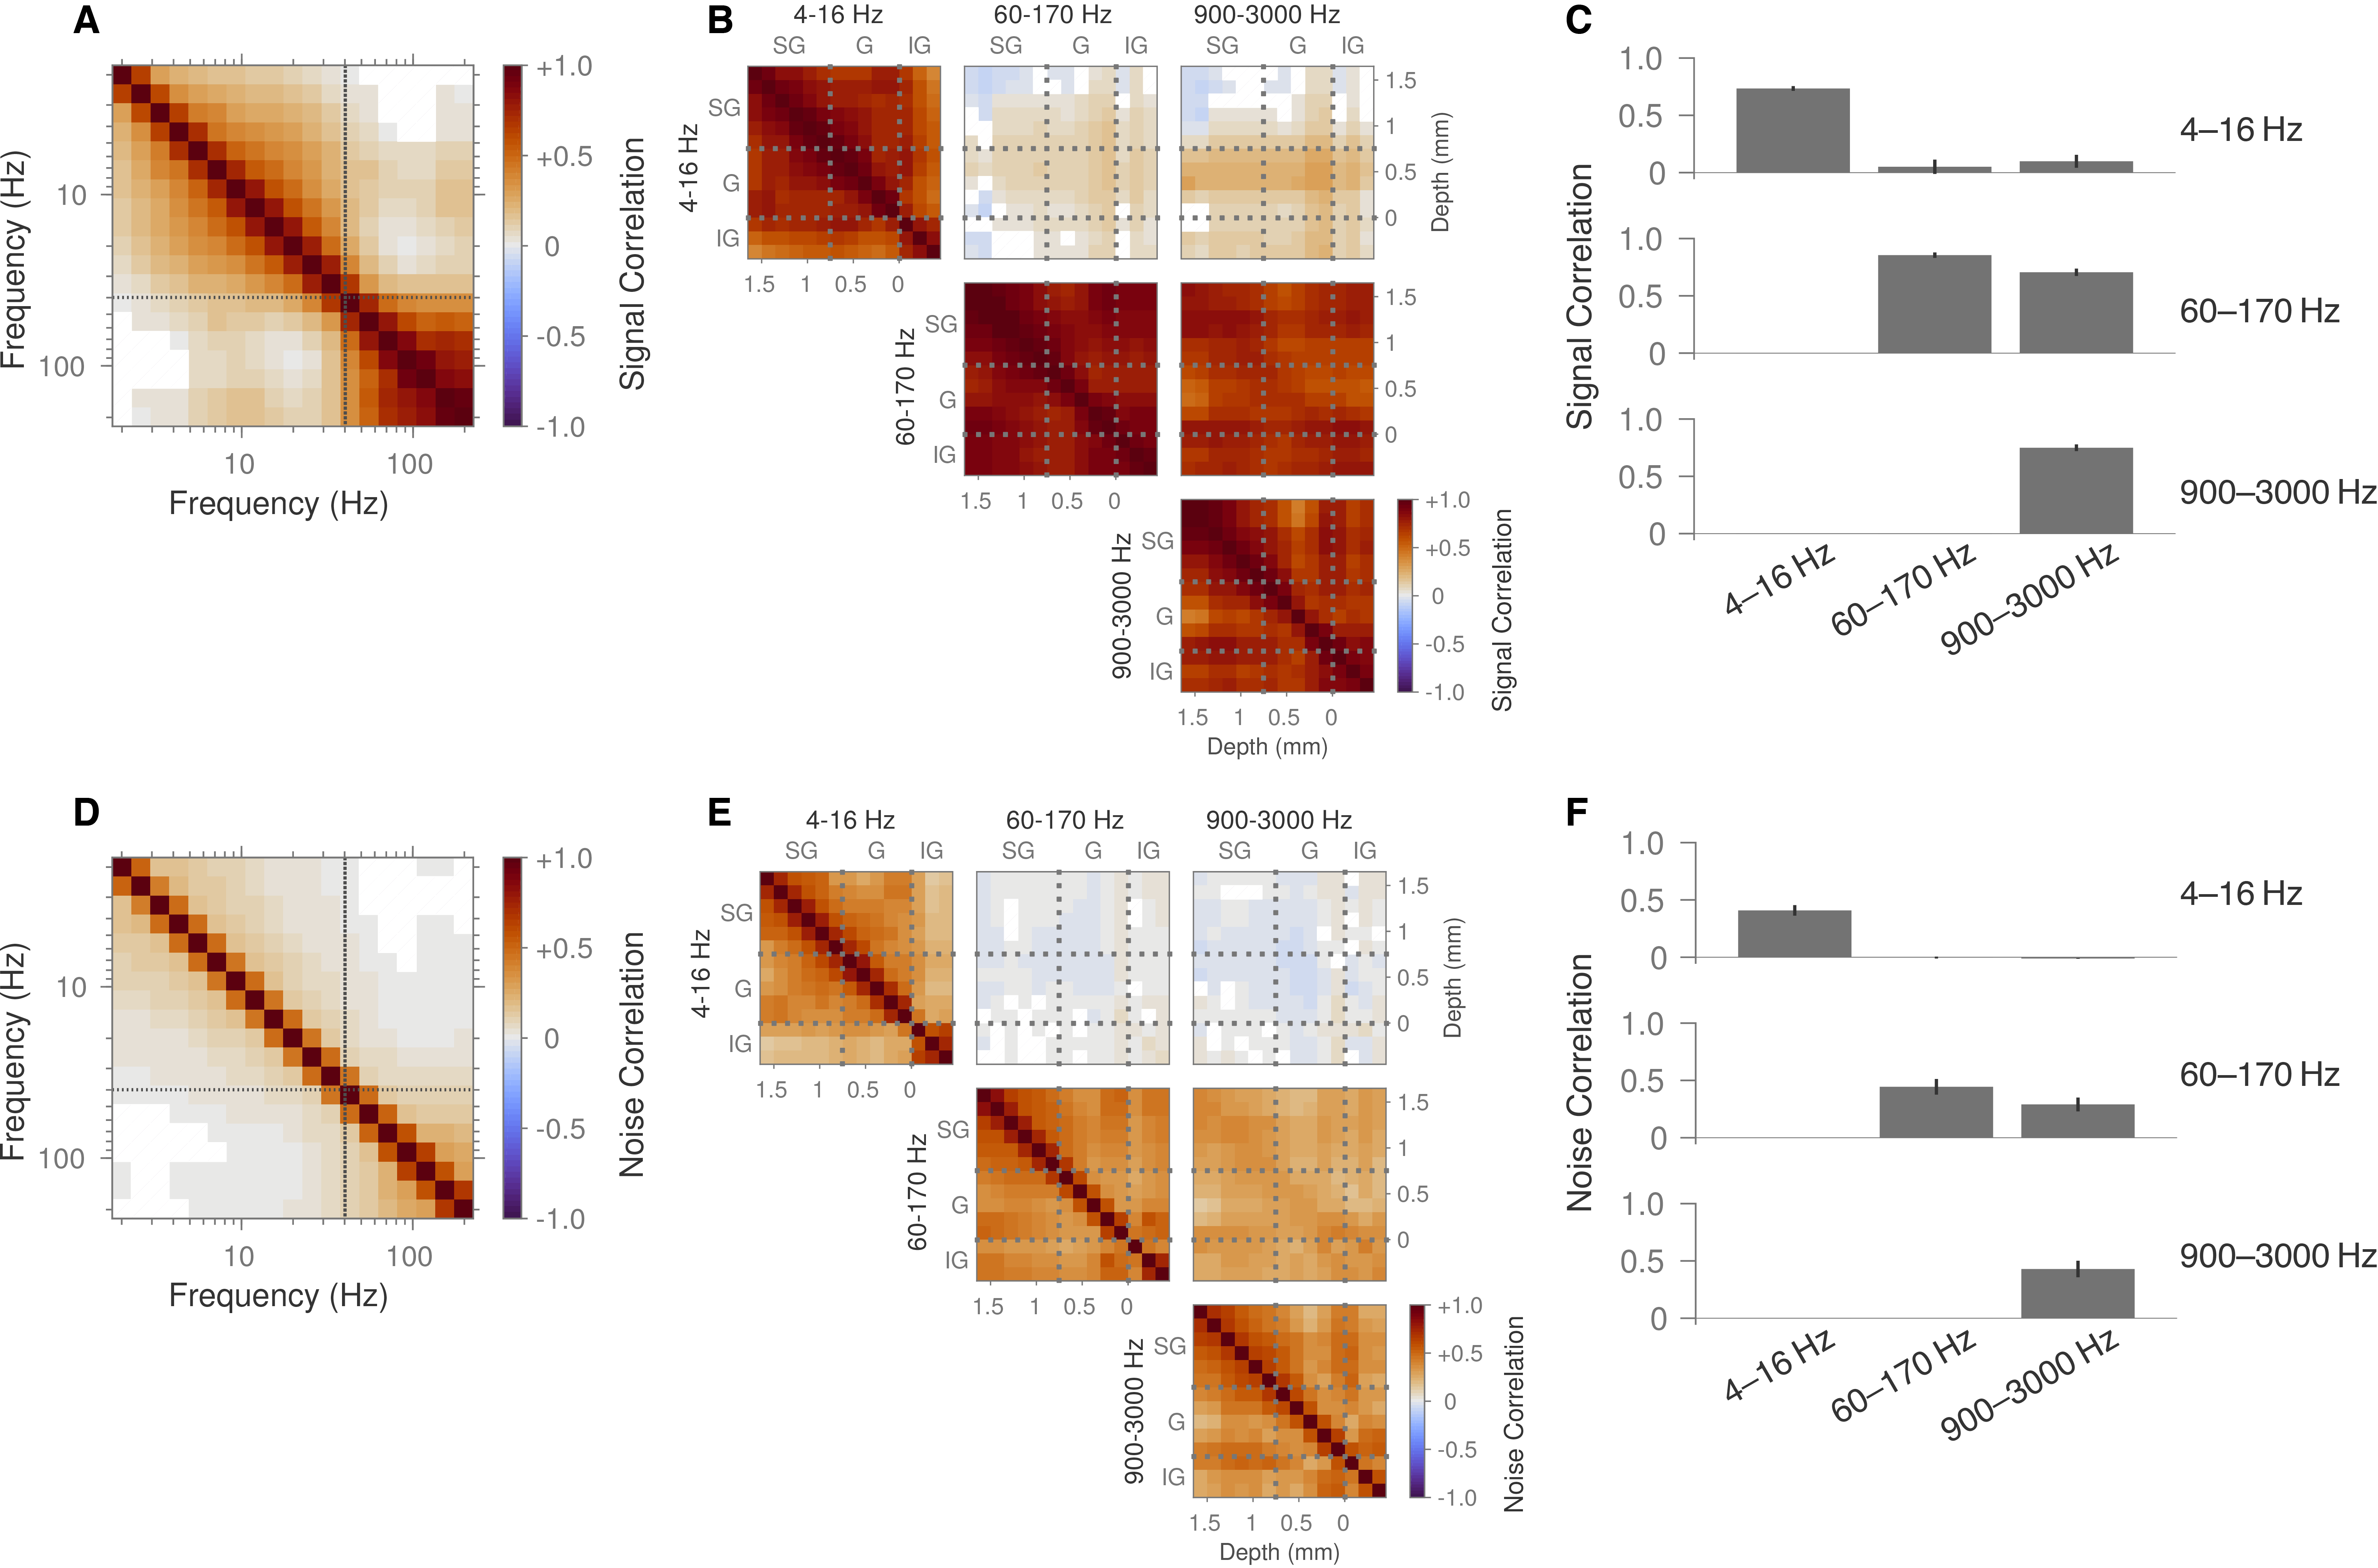
\includegraphics[width=\columnwidth]{paperfigs/figS3}
%
\caption{%
\textit{Signal and noise correlations.}
A: Median signal correlation between pairs of frequencies of the 14 recording sites, mean across 6 sessions.
Above, traces along the off-diagonals of the heatmap.
Each trace shows the redundancy between two bands with fixed ratio between their frequencies, against their geometric mean, with the shaded region indicating the standard error on the mean over 6 sessions.
B: Same as A, except for noise correlation instead of signal correlation.
C: Signal correlation between pairs of recording sites across the three frequency bands.
Mean of 6 sessions.
D: As C, but showing noise correlation.
E: Average signal correlation between each pair of frequency bands, found by averaging over all pairs of electrode contacts (excluding the trivial same-depth auto-correlation).
Error bars indicate the standard error over the 6 sessions.
F: As E, but showing noise correlation.
In A--D, datapoints which were not significantly different from the bootstrap mean (threshold at 3 standard deviations of bootstrapped correlation values) are shown in white.
The maximum upper and minimum lower thresholds employed for significance are shown on the colour bars.
Trivially correlated diagonal elements were removed (shown in black).
}
\label{fig:lam_s3}
%
\end{figure}


%\begin{figure}
%\centering \includegraphics[width=\columnwidth]{paperfigs/fig5S}
%%
%\caption{%
%\textit{Selection of number of bins.}
%We compare the amount of information in $N$ bins with the amount in $2N$ bins, and plot the percentage gain as a proportion of the amount of information found with $N$ bins.
%The threshold line (red) is set at \SI{5}{\percent}.
%Threshold is deemed to be exceeded when half the data falls below it.
%A: Mutual information between the ID of each frame, and the instantaneous power in the \ac{CSD} for band \SIrange{4}{16}{Hz} (Low; yellow) and band \SIrange{64}{250}{Hz} (High: purple), is shown against the number of bins for the band power.
%The frame ID is a unique identifier for each frame and hence does not need to be binned.
%B: Mutual information between the change in luminance between frames and the instantaneous power in the \ac{CSD} is shown against the number of bins for the change in luminance.
%The number of bins for the power band was fixed at 7.
%For "Coarse" the change in luminance is the \ac{RF} average, and for "Fine" it is the \ac{1}{px} scale change in luminance, minus the average.
%Frequency bands are the same as in A.
%}
%\label{fig:lam_s5}
%%
%\end{figure}


\begin{figure}
\centering 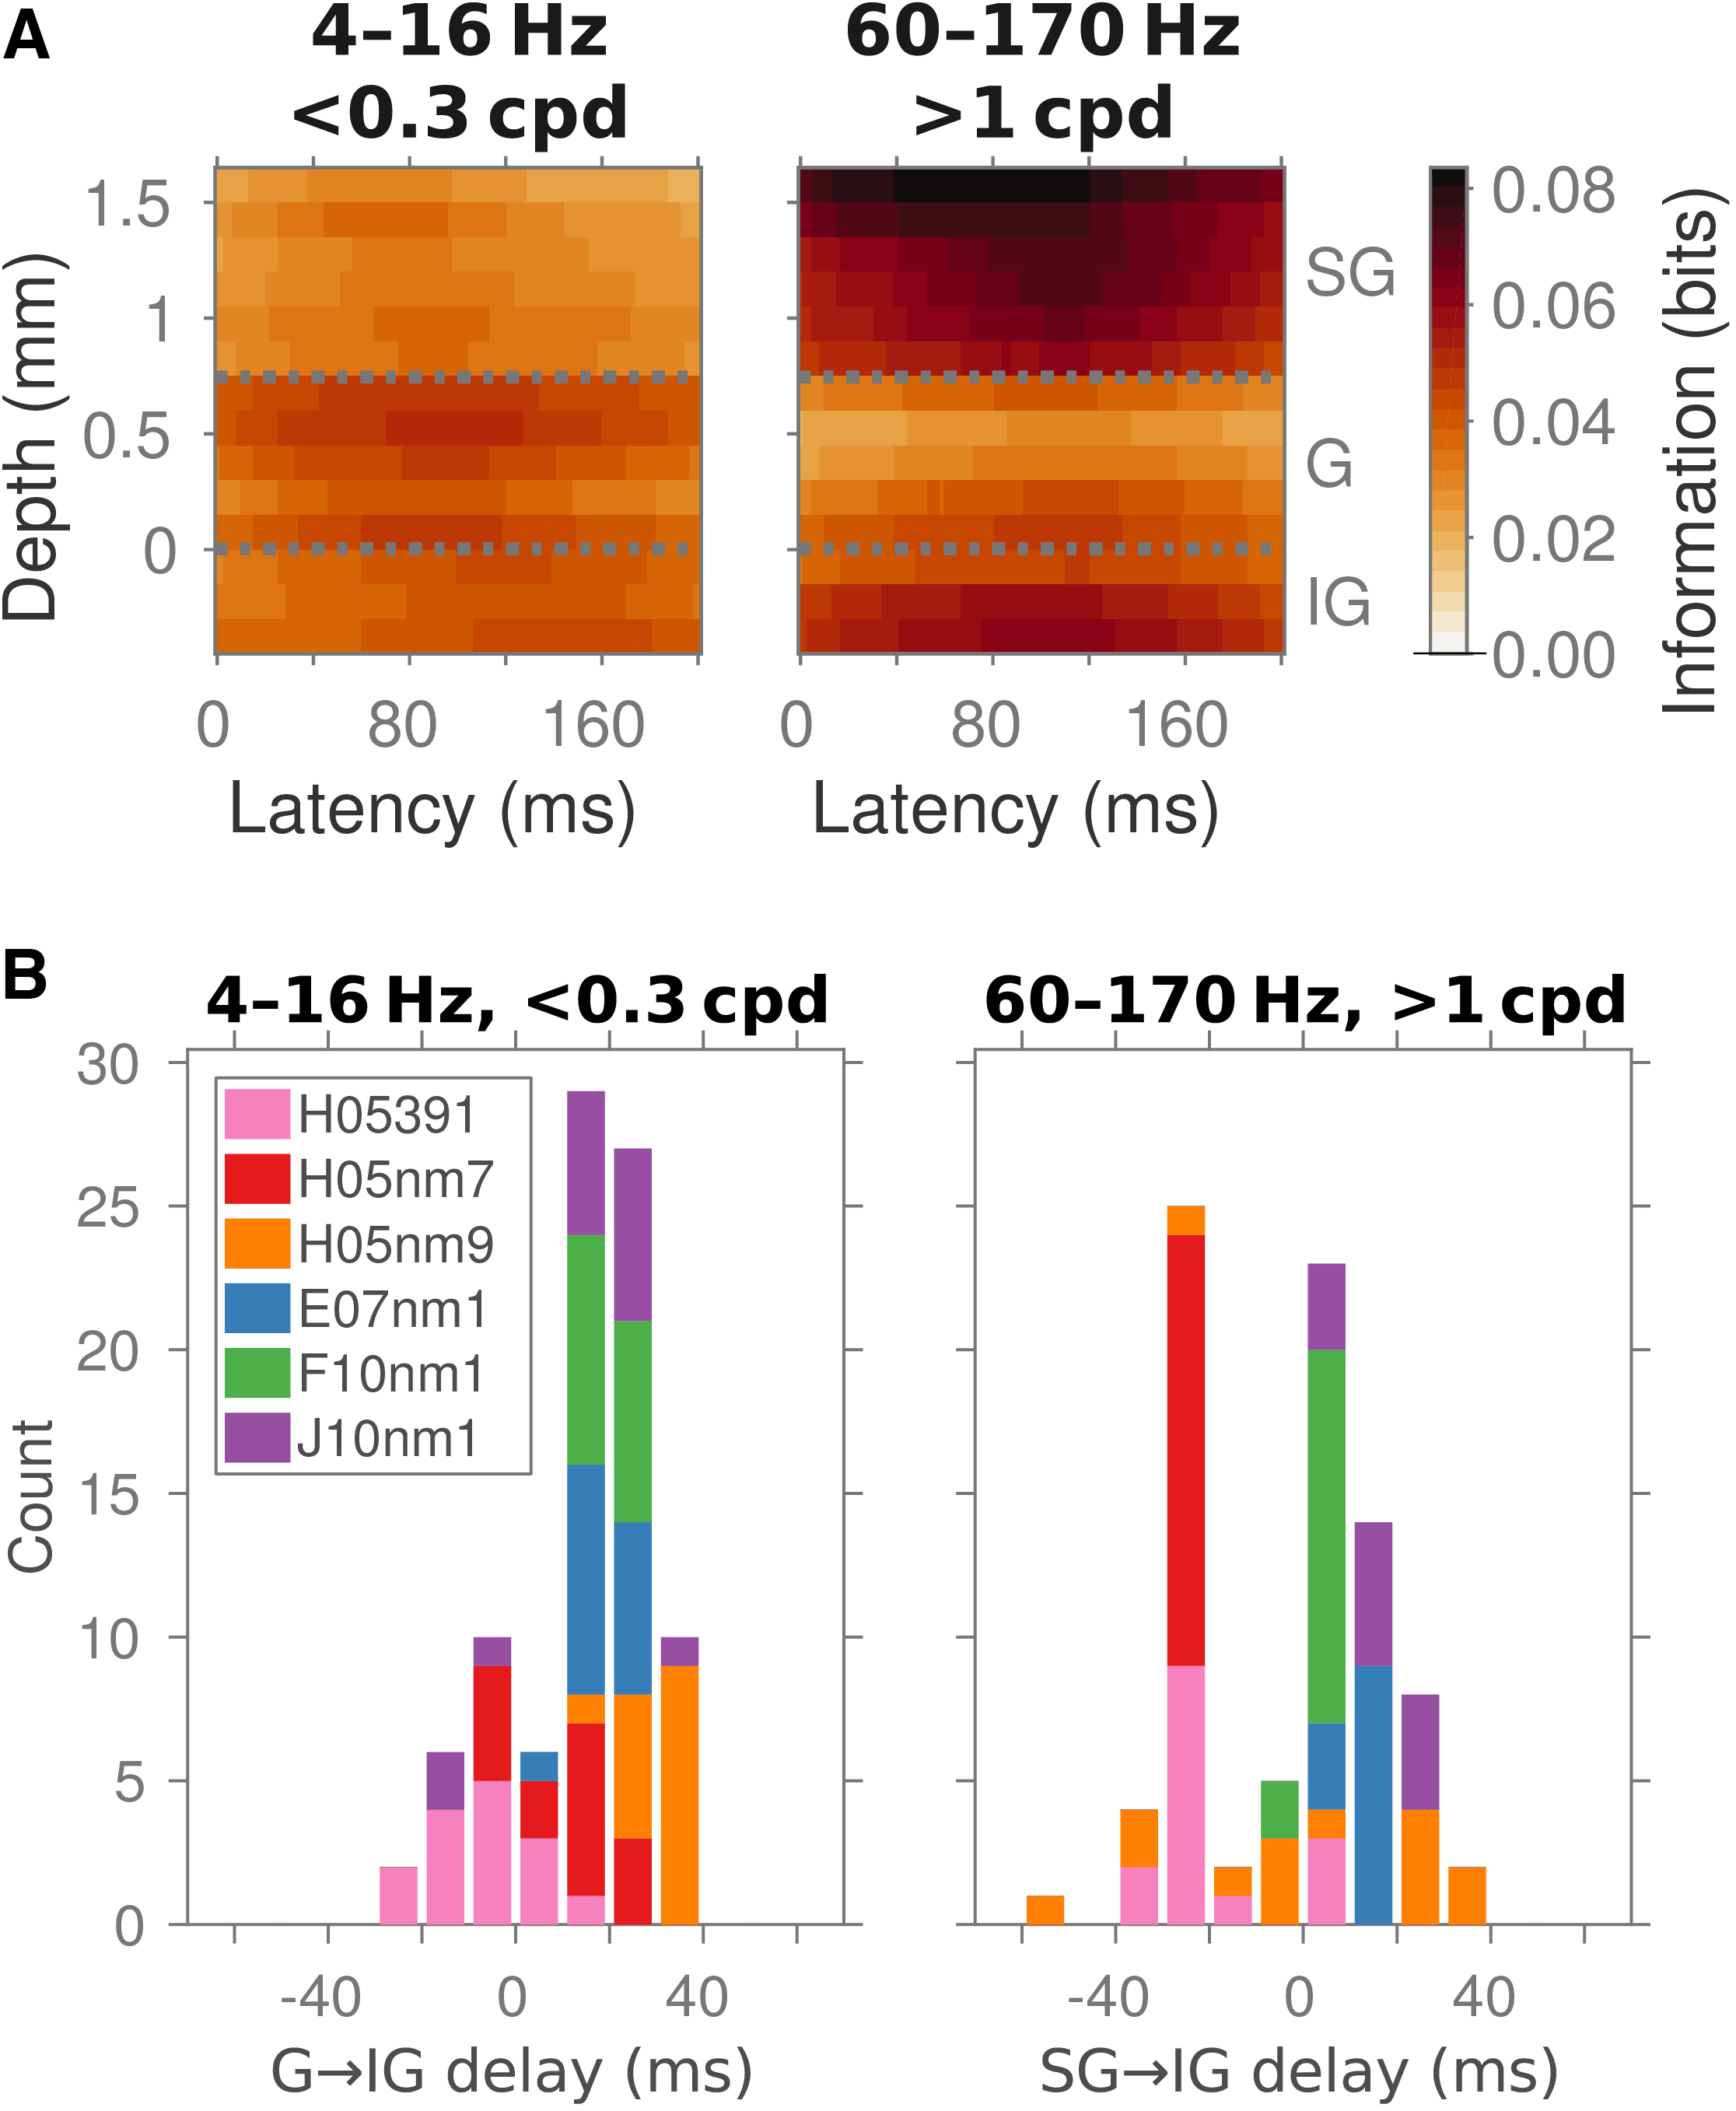
\includegraphics[width=\columnwidth]{paperfigs/figS6}
%
\caption{%
\textit{Latency of information.}
A: Information about the stimulus as a function of the prospective latency or lag between stimulus and response.
Left, information contained in \SIrange{4}{16}{Hz} power about \SI{<0.3}{\cpd} spatial components.
Right, information contained in \SIrange{60}{170}{Hz} power about \SI{>1}{\cpd} spatial components.
Mean of 6 sessions.
Each datapoint was tested for statistical significance using bootstrapping, and each datapoint was found to be significant.
B: Difference between pairs of depths for latency of maximum information.
Left, difference in peak-latency of information in \SIrange{4}{16}{Hz} power about \SI{<0.3}{\cpd} spatial components, between each electrode contact in \ac{G} and each in \ac{IG} compartments, for each recording session.
Right, difference in peak-latency of information in \SIrange{60}{170}{Hz} power about \SI{>1}{\cpd} spatial components, between each electrode contact in \ac{SG} and each in \ac{IG} compartments.
}
\label{fig:lam_s6}
%
\end{figure}


\FloatBarrier

\section{Supplemental Experimental Procedures}

\subsection{Aligning electrode penetrations}

For each recording session, the electrode was implanted in \iac{V1} at the recording site indicated in Supplemental \autoref{fig:lam_s1}A--B.
The methodology for the insertion of the electrode is described in the Experimental Methods of the main text.

For each penetration, we endeavoured to align the electrode such that the most shallow electrode contact was at the boundary between cortical matter and the dura (near \ac{L1}).
However, this \textit{ad-hoc} method of alignment is unreliable, in part due to variation in cortical and laminar thickness both within between subjects.
Therefore, we performed \textit{post-hoc} realignment of the electrode contacts using the same methodology as \citet{Self2013,VanKerkoerle2014}.

To identify the depth of each contact, we measured the potential evoked in response to the onset of the movie clip, and in response to full-screen maximum-luminance \SI{100}{\milli\second} flash stimuli with a \SI{6}{\second} interval.
From the measured potentials, we identified the boundary between the \ac{G} and \ac{IG} compartments as the source-sink reversal in the evoked \ac{CSD} \citep{Mitzdorf1979,Mitzdorf1985}.
For this measurement, the \ac{CSD} was computed from the \ac{LFP} as described in Experimental Methods, but without spatially smoothing the signal with a Hamming filter.

The data from each electrode was re-aligned such that the source-sink reversal for each recording session was at a depth of \SI{0}{\milli\metre} (\autoref{fig:lam_s1}C).
We estimated the location of the boundary between the \ac{G} and \ac{SG} compartments by cross-referencing literature describing the average thickness of cortical laminae in Macaca mulatta, area 17 \citep{Lund1973,OKusky1982}.

The validity of this choice of alignment of electrode penetrations was then tested by considering the average response in spiking activity to the onset of the stimulus, and by measuring the cortical thickness at the recording site using \ac{NMR}.

\subsubsection{Multi-unit spiking activity}

Spikes were detected by high-pass filtering the raw signal above \SI{500}{Hz} with a zero-phase eighth-order Butterworth filter, and classifying any points more than 3.5 standard deviations above the mean signal during pre- and post-stimulus periods as a spike, with a minimum inter-spike-interval of \SI{1}{\milli\second}.

The majority of thalamic afferents in \ac{V1} stimulate \ac{L4} (albeit indirectly, see \citealp{Hansen2012}), with the first cortical response manifesting at layer 4C$\alpha$ \citep{Callaway1998}, resulting in an initial current sink and first burst of spiking activity located here.
Consequently, we confirmed the depth alignment of the electrodes by verifying that the initial current sink (\autoref{fig:lam_s1}C) and spiking activity (\autoref{fig:lam_s1}D) in response to stimulation both resided within the \ac{G} compartment.

\subsubsection{Nuclear magnetic resonance data collection}

For two of the four monkeys involved in the study, we made use of high-resolution \ac{NMR} anatomical scans (collected for a different experiment) to measure the cortical thickness at the recording site used (Supplemental \autoref{fig:lam_s1}A--B).

To estimate the cortical thickness at the recording site of the laminar electrodes, high-resolution \ac{NMR} anatomical scans were acquired at the vertical using a \SI{7}{T} scanner with a \SI{60}{\centi\metre} diameter bore (Bruker BioSpin GmbH, Ettlingen, Germany).
A custom-made chair was used to position the monkey in the magnet.
We used a single-shot gradient \ac{EPI} with a \ac{FOV} of \SI{96x96}{\milli\metre} and matrix of \num{256x256}.
We acquired 18 a thickness of \SI{1}{\milli\metre}, TE/TR 15/\SI{2000}{\milli\second} and flip angle of \SI{90}{\degree}.

Animal \sesname{H05} was found to have a cortical thickness of \SI{\sim 1.7}{mm} at the recording site, whilst \sesname{E07} had a thickness of \SI{\sim 1.56}{mm}.

The thickness of cortical material included in the \ac{SG}, \ac{G} and \ac{IG} components is \SI{\sim 0.3}{mm} more than the measured obtained from the \ac{NMR} recordings.
We believe this discrepancy is due to the inflammation of the cortex in response to the trauma of the electrode penetration and the non-perpendicularity of the electrode penetration angle.


\subsection{Distribution of information across depth and frequency, per recording session}

The information about the stimulus contained in the power of the cortical oscillations was computed using the methodology described in the main text.
We present, in \autoref{fig:lam_s2}, the distribution of information in the power of \ac{CSD} oscillations as a function of depth and frequency for each experimental recording session.
The average over all sessions is shown in \autoref{fig:lam_2}.
The distribution of information is broadly the same for across all sessions --- highest in granular \SIrange{4}{16}{Hz} and supragranular \SIrange{60}{170}{Hz}, little information about the stimulus encoded in the intermediary \SIrange{20}{50}{Hz} range --- indicating our findings are reliable.


\subsection{Noise and signal correlations}

To accompany the information redundancy between frequencies and depths (\autoref{fig:lam_s3}), we also computed the noise and signal correlation between the power of oscillations (\autoref{fig:lam_s3}).

Both the signal and noise correlation show the same pattern across frequencies (\autoref{fig:lam_s3}A and D) as the information redundancy (\autoref{fig:lam_3}A), and similarly for the distribution across depth (\autoref{fig:lam_s3}B and E; \autoref{fig:lam_3}B).
However, the relationship is less clear for the signal and noise correlation than we observed for information redundancy.
For instance, since all signals are positively correlated in \autoref{fig:lam_s3}A (and D), the difference in correlation either side of the \SI{40}{Hz} line is less clear, though still evident.

Noise and signal correlation were both computed by binning the cortical response into bins of duration \SI{50}{\milli\second} following every frame change in the movie.

For the signal correlation, responses were averaged over repetitions to give a single mean response to each frame.
The set of cortical responses in a given frequency band and depth was correlated against the responses at another frequency band and depth using the Pearson correlation coefficient.

Noise correlation was computed by taking the set of responses in two different bands to a single frame onset and correlating their responses.
This was repeated for each frame, and the average over all frames was computed.

In each case, the analysis process was repeated with a shuffled pairing of responses in order to perform bootstrap statistics.
Correlation coefficients which were less than three standard deviations of the bootstraps from the bootstrap mean are shown as white in \autoref{fig:lam_s3}.
